% Dynamic Programming: Advanced
%
% Slides on dynamic programming considered too advanced for the introductory course.

\subsection{Dynamic Programming (advanced)}
\begin{frame}
  \frametitle{Gap Scoring}
  \begin{itemize}
    \item Simple gap penalty: all gaps score the same
    \begin{itemize}
      \item \emph{one} parameter in the alignment model
    \end{itemize}
    \item Affine gap penalty: opening and extending score differently
    \begin{itemize}
      \item \emph{two} parameters in the alignment model
    \end{itemize}
  \end{itemize}
  \begin{center}
    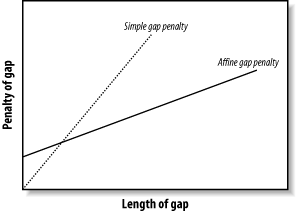
\includegraphics[width=0.3\textwidth]{images/gap_scores} 
  \end{center}
\end{frame}  
   
\begin{frame}
  \frametitle{Banded Alignment}
  \begin{itemize}
    \item Given a maximum scoring alignment, restrict search to a "band" between endpoints
    \item Width of this band = "bandwidth", another parameter in the model (may be floating)
    \item Speeds up search, reduces memory use
  \end{itemize}
  \begin{center}
    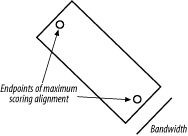
\includegraphics[width=0.3\textwidth]{images/banded} 
  \end{center}
\end{frame}     